\documentclass[a4paper, 11pt]{article}
\usepackage{comment} % enables the use of multi-line comments (\ifx \fi) 
\usepackage{fullpage} % changes the margin
\usepackage[a4paper, total={7in, 10in}]{geometry}
\usepackage{amsmath,mathtools}
\usepackage{amssymb,amsthm}  % assumes amsmath package installed
\usepackage{float}
\usepackage{xcolor}
\usepackage{mdframed}
\usepackage[shortlabels]{enumitem}
\usepackage{indentfirst}
\usepackage{hyperref}
\hypersetup{
	colorlinks=true,
	linkcolor=blue,
	filecolor=magenta,      
	urlcolor=blue!70!red,
	pdftitle={Assignment}, %%%%%%%%%%%%%%%%   WRITE ASSIGNMENT PDF NAME  %%%%%%%%%%%%%%%%%%%%
}
\usepackage[most,many,breakable]{tcolorbox}



\definecolor{mytheorembg}{HTML}{F2F2F9}
\definecolor{mytheoremfr}{HTML}{00007B}


\tcbuselibrary{theorems,skins,hooks}
\newtcbtheorem{problem}{Problem}
{%
	enhanced,
	breakable,
	colback = mytheorembg,
	frame hidden,
	boxrule = 0sp,
	borderline west = {2pt}{0pt}{mytheoremfr},
	sharp corners,
	detach title,
	before upper = \tcbtitle\par\smallskip,
	coltitle = mytheoremfr,
	fonttitle = \bfseries\sffamily,
	description font = \mdseries,
	separator sign none,
	segmentation style={solid, mytheoremfr},
}
{p}

% To give references for any problem use like this
% suppose the problem number is p3 then 2 options either 
% \hyperref[p:p3]{<text you want to use to hyperlink> \ref{p:p3}}
%                  or directly 
%                   \ref{p:p3}



%---------------------------------------
% BlackBoard Math Fonts :-
%---------------------------------------

%Captital Letters
\newcommand{\bbA}{\mathbb{A}}	\newcommand{\bbB}{\mathbb{B}}
\newcommand{\bbC}{\mathbb{C}}	\newcommand{\bbD}{\mathbb{D}}
\newcommand{\bbE}{\mathbb{E}}	\newcommand{\bbF}{\mathbb{F}}
\newcommand{\bbG}{\mathbb{G}}	\newcommand{\bbH}{\mathbb{H}}
\newcommand{\bbI}{\mathbb{I}}	\newcommand{\bbJ}{\mathbb{J}}
\newcommand{\bbK}{\mathbb{K}}	\newcommand{\bbL}{\mathbb{L}}
\newcommand{\bbM}{\mathbb{M}}	\newcommand{\bbN}{\mathbb{N}}
\newcommand{\bbO}{\mathbb{O}}	\newcommand{\bbP}{\mathbb{P}}
\newcommand{\bbQ}{\mathbb{Q}}	\newcommand{\bbR}{\mathbb{R}}
\newcommand{\bbS}{\mathbb{S}}	\newcommand{\bbT}{\mathbb{T}}
\newcommand{\bbU}{\mathbb{U}}	\newcommand{\bbV}{\mathbb{V}}
\newcommand{\bbW}{\mathbb{W}}	\newcommand{\bbX}{\mathbb{X}}
\newcommand{\bbY}{\mathbb{Y}}	\newcommand{\bbZ}{\mathbb{Z}}

%---------------------------------------
% MathCal Fonts :-
%---------------------------------------

%Captital Letters
\newcommand{\mcA}{\mathcal{A}}	\newcommand{\mcB}{\mathcal{B}}
\newcommand{\mcC}{\mathcal{C}}	\newcommand{\mcD}{\mathcal{D}}
\newcommand{\mcE}{\mathcal{E}}	\newcommand{\mcF}{\mathcal{F}}
\newcommand{\mcG}{\mathcal{G}}	\newcommand{\mcH}{\mathcal{H}}
\newcommand{\mcI}{\mathcal{I}}	\newcommand{\mcJ}{\mathcal{J}}
\newcommand{\mcK}{\mathcal{K}}	\newcommand{\mcL}{\mathcal{L}}
\newcommand{\mcM}{\mathcal{M}}	\newcommand{\mcN}{\mathcal{N}}
\newcommand{\mcO}{\mathcal{O}}	\newcommand{\mcP}{\mathcal{P}}
\newcommand{\mcQ}{\mathcal{Q}}	\newcommand{\mcR}{\mathcal{R}}
\newcommand{\mcS}{\mathcal{S}}	\newcommand{\mcT}{\mathcal{T}}
\newcommand{\mcU}{\mathcal{U}}	\newcommand{\mcV}{\mathcal{V}}
\newcommand{\mcW}{\mathcal{W}}	\newcommand{\mcX}{\mathcal{X}}
\newcommand{\mcY}{\mathcal{Y}}	\newcommand{\mcZ}{\mathcal{Z}}



%---------------------------------------
% Bold Math Fonts :-
%---------------------------------------

%Captital Letters
\newcommand{\bmA}{\boldsymbol{A}}	\newcommand{\bmB}{\boldsymbol{B}}
\newcommand{\bmC}{\boldsymbol{C}}	\newcommand{\bmD}{\boldsymbol{D}}
\newcommand{\bmE}{\boldsymbol{E}}	\newcommand{\bmF}{\boldsymbol{F}}
\newcommand{\bmG}{\boldsymbol{G}}	\newcommand{\bmH}{\boldsymbol{H}}
\newcommand{\bmI}{\boldsymbol{I}}	\newcommand{\bmJ}{\boldsymbol{J}}
\newcommand{\bmK}{\boldsymbol{K}}	\newcommand{\bmL}{\boldsymbol{L}}
\newcommand{\bmM}{\boldsymbol{M}}	\newcommand{\bmN}{\boldsymbol{N}}
\newcommand{\bmO}{\boldsymbol{O}}	\newcommand{\bmP}{\boldsymbol{P}}
\newcommand{\bmQ}{\boldsymbol{Q}}	\newcommand{\bmR}{\boldsymbol{R}}
\newcommand{\bmS}{\boldsymbol{S}}	\newcommand{\bmT}{\boldsymbol{T}}
\newcommand{\bmU}{\boldsymbol{U}}	\newcommand{\bmV}{\boldsymbol{V}}
\newcommand{\bmW}{\boldsymbol{W}}	\newcommand{\bmX}{\boldsymbol{X}}
\newcommand{\bmY}{\boldsymbol{Y}}	\newcommand{\bmZ}{\boldsymbol{Z}}
%Small Letters
\newcommand{\bma}{\boldsymbol{a}}	\newcommand{\bmb}{\boldsymbol{b}}
\newcommand{\bmc}{\boldsymbol{c}}	\newcommand{\bmd}{\boldsymbol{d}}
\newcommand{\bme}{\boldsymbol{e}}	\newcommand{\bmf}{\boldsymbol{f}}
\newcommand{\bmg}{\boldsymbol{g}}	\newcommand{\bmh}{\boldsymbol{h}}
\newcommand{\bmi}{\boldsymbol{i}}	\newcommand{\bmj}{\boldsymbol{j}}
\newcommand{\bmk}{\boldsymbol{k}}	\newcommand{\bml}{\boldsymbol{l}}
\newcommand{\bmm}{\boldsymbol{m}}	\newcommand{\bmn}{\boldsymbol{n}}
\newcommand{\bmo}{\boldsymbol{o}}	\newcommand{\bmp}{\boldsymbol{p}}
\newcommand{\bmq}{\boldsymbol{q}}	\newcommand{\bmr}{\boldsymbol{r}}
\newcommand{\bms}{\boldsymbol{s}}	\newcommand{\bmt}{\boldsymbol{t}}
\newcommand{\bmu}{\boldsymbol{u}}	\newcommand{\bmv}{\boldsymbol{v}}
\newcommand{\bmw}{\boldsymbol{w}}	\newcommand{\bmx}{\boldsymbol{x}}
\newcommand{\bmy}{\boldsymbol{y}}	\newcommand{\bmz}{\boldsymbol{z}}

%---------------------------------------
% Scr Math Fonts :-
%---------------------------------------

\newcommand{\sA}{{\mathscr{A}}}   \newcommand{\sB}{{\mathscr{B}}}
\newcommand{\sC}{{\mathscr{C}}}   \newcommand{\sD}{{\mathscr{D}}}
\newcommand{\sE}{{\mathscr{E}}}   \newcommand{\sF}{{\mathscr{F}}}
\newcommand{\sG}{{\mathscr{G}}}   \newcommand{\sH}{{\mathscr{H}}}
\newcommand{\sI}{{\mathscr{I}}}   \newcommand{\sJ}{{\mathscr{J}}}
\newcommand{\sK}{{\mathscr{K}}}   \newcommand{\sL}{{\mathscr{L}}}
\newcommand{\sM}{{\mathscr{M}}}   \newcommand{\sN}{{\mathscr{N}}}
\newcommand{\sO}{{\mathscr{O}}}   \newcommand{\sP}{{\mathscr{P}}}
\newcommand{\sQ}{{\mathscr{Q}}}   \newcommand{\sR}{{\mathscr{R}}}
\newcommand{\sS}{{\mathscr{S}}}   \newcommand{\sT}{{\mathscr{T}}}
\newcommand{\sU}{{\mathscr{U}}}   \newcommand{\sV}{{\mathscr{V}}}
\newcommand{\sW}{{\mathscr{W}}}   \newcommand{\sX}{{\mathscr{X}}}
\newcommand{\sY}{{\mathscr{Y}}}   \newcommand{\sZ}{{\mathscr{Z}}}


%---------------------------------------
% Math Fraktur Font
%---------------------------------------

%Captital Letters
\newcommand{\mfA}{\mathfrak{A}}	\newcommand{\mfB}{\mathfrak{B}}
\newcommand{\mfC}{\mathfrak{C}}	\newcommand{\mfD}{\mathfrak{D}}
\newcommand{\mfE}{\mathfrak{E}}	\newcommand{\mfF}{\mathfrak{F}}
\newcommand{\mfG}{\mathfrak{G}}	\newcommand{\mfH}{\mathfrak{H}}
\newcommand{\mfI}{\mathfrak{I}}	\newcommand{\mfJ}{\mathfrak{J}}
\newcommand{\mfK}{\mathfrak{K}}	\newcommand{\mfL}{\mathfrak{L}}
\newcommand{\mfM}{\mathfrak{M}}	\newcommand{\mfN}{\mathfrak{N}}
\newcommand{\mfO}{\mathfrak{O}}	\newcommand{\mfP}{\mathfrak{P}}
\newcommand{\mfQ}{\mathfrak{Q}}	\newcommand{\mfR}{\mathfrak{R}}
\newcommand{\mfS}{\mathfrak{S}}	\newcommand{\mfT}{\mathfrak{T}}
\newcommand{\mfU}{\mathfrak{U}}	\newcommand{\mfV}{\mathfrak{V}}
\newcommand{\mfW}{\mathfrak{W}}	\newcommand{\mfX}{\mathfrak{X}}
\newcommand{\mfY}{\mathfrak{Y}}	\newcommand{\mfZ}{\mathfrak{Z}}
%Small Letters
\newcommand{\mfa}{\mathfrak{a}}	\newcommand{\mfb}{\mathfrak{b}}
\newcommand{\mfc}{\mathfrak{c}}	\newcommand{\mfd}{\mathfrak{d}}
\newcommand{\mfe}{\mathfrak{e}}	\newcommand{\mff}{\mathfrak{f}}
\newcommand{\mfg}{\mathfrak{g}}	\newcommand{\mfh}{\mathfrak{h}}
\newcommand{\mfi}{\mathfrak{i}}	\newcommand{\mfj}{\mathfrak{j}}
\newcommand{\mfk}{\mathfrak{k}}	\newcommand{\mfl}{\mathfrak{l}}
\newcommand{\mfm}{\mathfrak{m}}	\newcommand{\mfn}{\mathfrak{n}}
\newcommand{\mfo}{\mathfrak{o}}	\newcommand{\mfp}{\mathfrak{p}}
\newcommand{\mfq}{\mathfrak{q}}	\newcommand{\mfr}{\mathfrak{r}}
\newcommand{\mfs}{\mathfrak{s}}	\newcommand{\mft}{\mathfrak{t}}
\newcommand{\mfu}{\mathfrak{u}}	\newcommand{\mfv}{\mathfrak{v}}
\newcommand{\mfw}{\mathfrak{w}}	\newcommand{\mfx}{\mathfrak{x}}
\newcommand{\mfy}{\mathfrak{y}}	\newcommand{\mfz}{\mathfrak{z}}

%---------------------------------------
% Bar
%---------------------------------------

%Captital Letters
\newcommand{\barA}{\overline{A}}	\newcommand{\barB}{\overline{B}}
\newcommand{\barC}{\overline{C}}	\newcommand{\barD}{\overline{D}}
\newcommand{\barE}{\overline{E}}	\newcommand{\barF}{\overline{F}}
\newcommand{\barG}{\overline{G}}	\newcommand{\barH}{\overline{H}}
\newcommand{\barI}{\overline{I}}	\newcommand{\barJ}{\overline{J}}
\newcommand{\barK}{\overline{K}}	\newcommand{\barL}{\overline{L}}
\newcommand{\barM}{\overline{M}}	\newcommand{\barN}{\overline{N}}
\newcommand{\barO}{\overline{O}}	\newcommand{\barP}{\overline{P}}
\newcommand{\barQ}{\overline{Q}}	\newcommand{\barR}{\overline{R}}
\newcommand{\barS}{\overline{S}}	\newcommand{\barT}{\overline{T}}
\newcommand{\barU}{\overline{U}}	\newcommand{\barV}{\overline{V}}
\newcommand{\barW}{\overline{W}}	\newcommand{\barX}{\overline{X}}
\newcommand{\barY}{\overline{Y}}	\newcommand{\barZ}{\overline{Z}}
%Small Letters
\newcommand{\bara}{\overline{a}}	\newcommand{\barb}{\overline{b}}
\newcommand{\barc}{\overline{c}}	\newcommand{\bard}{\overline{d}}
\newcommand{\bare}{\overline{e}}	\newcommand{\barf}{\overline{f}}
\newcommand{\barg}{\overline{g}}	\newcommand{\barh}{\overline{h}}
\newcommand{\bari}{\overline{i}}	\newcommand{\barj}{\overline{j}}
\newcommand{\bark}{\overline{k}}	\newcommand{\barl}{\overline{l}}
\newcommand{\barm}{\overline{m}}	\newcommand{\barn}{\overline{n}}
\newcommand{\baro}{\overline{o}}	\newcommand{\barp}{\overline{p}}
\newcommand{\barq}{\overline{q}}	\newcommand{\barr}{\overline{r}}
\newcommand{\bars}{\overline{s}}	\newcommand{\bart}{\overline{t}}
\newcommand{\baru}{\overline{u}}	\newcommand{\barv}{\overline{v}}
\newcommand{\barw}{\overline{w}}	\newcommand{\barx}{\overline{x}}
\newcommand{\bary}{\overline{y}}	\newcommand{\barz}{\overline{z}}

%---------------------------------------
% Greek Letters:-
%---------------------------------------
\newcommand{\eps}{\epsilon}
\newcommand{\veps}{\varepsilon}
\newcommand{\lm}{\lambda}
\newcommand{\Lm}{\Lambda}
\newcommand{\gm}{\gamma}
\newcommand{\Gm}{\Gamma}
\newcommand{\vph}{\varphi}
\newcommand{\ph}{\phi}

\newcommand{\Qed}{\begin{flushright}\qed\end{flushright}}
\newcommand{\parinn}{\setlength{\parindent}{1cm}}
\newcommand{\parinf}{\setlength{\parindent}{0cm}}
\newcommand{\del}[2]{\frac{\partial #1}{\partial #2}}
\newcommand{\Del}[3]{\frac{\partial^{#1} #2}{\partial^{#1} #3}}
\newcommand{\deld}[2]{\dfrac{\partial #1}{\partial #2}}
\newcommand{\Deld}[3]{\dfrac{\partial^{#1} #2}{\partial^{#1} #3}}
\newcommand{\uin}{\mathbin{\rotatebox[origin=c]{90}{$\in$}}}
\newcommand{\usubset}{\mathbin{\rotatebox[origin=c]{90}{$\subset$}}}
\newcommand{\lt}{\left}
\newcommand{\rt}{\right}
\newcommand{\exs}{\exists}
\newcommand{\st}{\strut}
\newcommand{\dps}[1]{\displaystyle{#1}}
\newcommand{\la}{\langle}
\newcommand{\ra}{\rangle}
\newenvironment{solution}
{\textit{\textbf{Solution:}} 
}
{ 
	\hfill $\blacksquare$
	
	\vspace{1cm}
}
\newcommand{\sol}[1]{\begin{solution}#1\end{solution}}
\newcommand{\solve}[1]{\setlength{\parindent}{0cm}\textbf{\textit{Solution: }}\setlength{\parindent}{1cm}#1 \Qed}
\newcommand{\mat}[1]{\left[\begin{matrix}#1\end{matrix}\right]}
\newcommand\numberthis{\addtocounter{equation}{1}\tag{\theequation}}
\newcommand{\handout}[3]{
	\noindent
	\begin{center}
		\framebox{
			\vbox{
				\hbox to 6.5in { {\bf Complexity Theory I } \hfill Jan -- May, 2023 }
				\vspace{4mm}
				\hbox to 6.5in { {\Large \hfill #1  \hfill} }
				\vspace{2mm}
				\hbox to 6.5in { {\em #2 \hfill #3} }
			}
		}
	\end{center}
	\vspace*{4mm}
}

\newcommand{\lecture}[3]{\handout{Lecture #1}{Lecturer: #2}{Scribe:	#3}}
	

\newcommand{\ov}[1]{\overline{#1}}
\newcommand{\thmref}[1]{\hyperref[#1]{Theorem \ref{#1}}}

\setlength{\parindent}{0pt}

%%%%%%%%%%%%%%%%%%%%%%%%%%%%%%%%%%%%%%%%%%%%%%%%%%%%%%%%%%%%%%%%%%%%%%%%%%%%%%%%%%%%%%%%%%%%%%%%%%%%%%%%%%%%%%%%%%%%%%%%%%%%%%%%%%%%%%%%

\begin{document}
	
	%%%%%%%%%%%%%%%%%%%%%%%%%%%%%%%%%%%%%%%%%%%%%%%%%%%%%%%%%%%%%%%%%%%%%%%%%%%%%%%%%%%%%%%%%%%%%%%%%%%%%%%%%%%%%%%%%%%%%%%%%%%%%%%%%%%%%%%%
	
	\textsf{\noindent \large\textbf{Soham Chatterjee} \hfill \textbf{Assignment - 2}\\
		Email: \href{sohamc@cmi.ac.in}{sohamc@cmi.ac.in} \hfill Roll: BMC202175\\
		\normalsize Course: Complex Analysis \hfill Date: February 9, 2023}
	
	%%%%%%%%%%%%%%%%%%%%%%%%%%%%%%%%%%%%%%%%%%%%%%%%%%%%%%%%%%%%%%%%%%%%%%%%%%%%%%%%%%%%%%%%%%%%%%%%%%%%%%%%%%%%%%%%%%%%%%%%%%%%%%%%%%%%%%%%
	% Problem 1
	%%%%%%%%%%%%%%%%%%%%%%%%%%%%%%%%%%%%%%%%%%%%%%%%%%%%%%%%%%%%%%%%%%%%%%%%%%%%%%%%%%%%%%%%%%%%%%%%%%%%%%%%%%%%%%%%%%%%%%%%%%%%%%%%%%%%%%%%
	
	\begin{problem}{%problem statement
			Ahlfors Page 47: Problem 1
		}{p1% problem reference text
		}
	For real $y$ show that every remainder in the series for $\cos y$ and $\sin y$ has the same sign as the leading term
		%Problem		
	\end{problem}
	
	\solve{
		%Solution
		The series for both cosine and sine are
		$$
		\begin{aligned}
			\cos (y) & =\sum_{k=0}^{\infty}(-1)^k \frac{y^{2 k}}{(2 k) !} =1-\frac{y^2}{2 !}+\frac{y^4}{4 !}-\cdots \\
			\sin (y) & =\sum_{k=0}^{\infty}(-1)^k \frac{y^{2 k+1}}{(2 k+1) !} =y-\frac{y^3}{3 !}+\frac{y^6}{6 !}-\cdots
		\end{aligned}
		$$
		We can write Taylor's formula as $f(y)=T_n(y)+R_n(y)$ where
		$$
		f(y)=\sum_{k=0}^n \frac{f^{(k)}(0)}{k !} y^k+\frac{1}{k !} \int_0^y(y-t)^k f^{(k+1)}(t) d t .
		$$
		Now, we can write cosine and sine of $y$ as
		$$
		\begin{aligned}
			& \cos (y)=\sum_{k=0}^n \frac{(-1)^k y^{2 k}}{(2 k) !}+\frac{1}{n !} \int_0^y(y-t)^n \cos ^{n+1}(t) d t \\
			& \sin (y)=\sum_{k=0}^{n-1} \frac{(-1)^k y^{2 k+1}}{(2 k+1) !}+\frac{1}{n !} \int_0^y(y-t)^n \sin ^n(t) d t
		\end{aligned}
		$$
		Now we have $$\sin^{(2m)}(t)=(-1)^m\sin t\qquad \cos^{(2m+1)}(t)=(-1)^{m+1}\sin t$$For cosine and sine, let $n=2 m$ and $n=2 m-1$, respectively. Then
		\begin{align*}
			 \cos (y)& =\sum_{k=0}^m \frac{(-1)^k y^{2 k}}{(2 k) !}+\frac{1}{(2 m) !} \int_0^y(y-t)^{2 m} \cos ^{2 m+1}(t) d t \\
			& =\sum_{k=0}^m \frac{(-1)^k}{(2k)!}y^{2k} + \frac{(-1)^{m+1}}{(2m)!} \int_0^y (y-t)^{2m} \sin tdt\\
			\\
			 \sin (y)& =\sum_{k=0}^{m-1} \frac{(-1)^k y^{2 k+1}}{(2 k+1) !}+\frac{1}{(2 m-1) !} \int_0^y(y-t)^{2 m-1} \sin ^{2 m-1}(t) d t\\
			 & =\sum_{k=0}^{m-1} \frac{(-1)^k}{(2k+1)!}y^{2k+1} + \frac{(-1)^m}{(2m-1)!} \int_0^y (y-t)^{2m-1}\sin tdt
		\end{align*}
	So it remains to see that
	
	$$\int_0^y (y-t)^k \sin t\, dt > 0$$for all $y > 0$ and $k > 0$. But that follows since $(y-t)^k$ is a strictly decreasing positive function, so while $2p\pi  \leqslant y$ where $p\in \bbN$ we have
	
	$$
		\int_{2n\pi}^{2(n+1)\pi} (y-t)^k\sin t\,dt = \underbrace{\int_{2n\pi}^{(2n+1)\pi} \underbrace{(y-t)^k}_{>0}\underbrace{\sin t}_{>0}\,dt}_{>0}+\underbrace{\int^{2(n+1)\pi}_{(2n+1)\pi} \underbrace{(y-t)^k}_{>0}\underbrace{\sin t}_{<0}\,dt}_{<0}$$Now \begin{align*}
			\int_{2n\pi}^{(2n+1)\pi} {(y-t)^k}{\sin t}\,dt & > (y-(2n+1)\pi)^k\int^{2(n+1)\pi}_{2n\pi}\sin t\, dt\\
			&= 2 (y-(2n+1)\pi)^k\\ 
			\\
			\int^{2(n+1)\pi}_{(2n+1)\pi} {(y-t)^k}{\sin t}\,dt & =-\int^{2(n+1)\pi}_{(2n+1)\pi} \underbrace{(y-t)^k}_{>0}\underbrace{(-\sin t)}_{>0}\,dt\\ &>-(y-(2n+1)\pi)^k\int^{2(n+1)\pi}_{(2n+1)\pi}(-\sin t)dt\\
			& = -2(y-(2n+1)\pi)^k
	\end{align*}Hence $$	\int_{2n\pi}^{2(n+1)\pi} (y-t)^k\sin t\,dt>0$$This is true for all $n\in \{0,1,\dots,p\}$. Therefore $$\int_0^{2p\pi} (y-t)^k \sin t\, dt > 0$$Now if $2p\pi\leq y\leq (2p+1)\pi$ then $$\int_{2p\pi}^y (y-t)^k\sin t\,dt\geq 0$$If $(2p+1)\pi\leq y\leq 2(p+1)\pi$
	
	\begin{align*}
		\int_{2p\pi}^y (y-t)^k\sin t\,dt &= \int_{2p\pi}^{(2p+1)\pi}(y-t)^k\sin t\,dt + \int_{(2p+1)\pi}^y(y-t)^k\lvert\sin t\rvert\,dt\\
		&= \int_{2p\pi}^{(2p+1)\pi}(y-t)^k\sin t\,dt + \int_{(2p+1)\pi}^{2(p+1)\pi}(y-t)^k\lvert\sin t\rvert\,dt\\
		&> (y-(2p+1)\pi)^k \int_0^\pi\sin t\,dt - (y-(2p+1)\pi)^k\int_{(2p+1)\pi}^{2(p+1)\pi}\sin t\,dt\\
		&> 0
	\end{align*}
		
	}
	
	
	%%%%%%%%%%%%%%%%%%%%%%%%%%%%%%%%%%%%%%%%%%%%%%%%%%%%%%%%%%%%%%%%%%%%%%%%%
	% Problem 2
	%%%%%%%%%%%%%%%%%%%%%%%%%%%%%%%%%%%%%%%%%%%%%%%%%%%%%%%%%%%%%%%%%%%%%%%%%
	
	\begin{problem}{%problem statement
			Ahlfors Page 47: Problem 2
		}{p2% problem reference text
		}
		%Problem		
		Prove, for instance that $3<\pi< 2\sqrt{3}$
	\end{problem}
	
	\solve{
		%Solution
	\begin{center}
		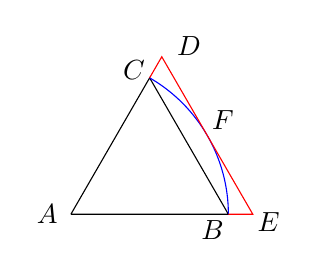
\begin{tikzpicture}
			\draw (0,0) node[xshift=-3mm] {$A$} -- (2,0)node[xshift=-2mm,yshift=-2mm] {$B$} -- (1,1.732) node[xshift=-2mm,yshift=1mm] {$C$} -- (0,0);
			\draw[blue] (2,0) arc (0:60:2);
			\draw[red] (1,1.732) node[xshift=5mm,yshift=4mm,color=black]{$D$} -- (1.154,2) -- (2.31,0)node[xshift=2mm,yshift=-1mm,color=black]{$E$} -- (2,0);
			\draw (1.732,1) node[xshift=2mm,yshift=2mm]{$F$};
		\end{tikzpicture}
	\end{center}
The triangles $\triangle ABC$ and $\triangle DAE$ are equilateral triangles. Side length of $\triangle ABC$ is 1. The radius of the circular sector $ACFBA$ is 1. Hence the height of the triangle $\triangle ADE$ is 1. Therefore the side length of the $\triangle ADE$ is $\frac2{\sqrt{3}}$. Now the arc length of $BFC$ is greater than the side length of the triangle $\triangle ABC$. Therefore $$\frac{2\times \pi \times  1}{6} > 1\implies \pi > 3$$So the we have $$ Area(ABFCA) < Area (\triangle ADE)$$ Now,  $Area(ABFCA)=\frac16 \, \pi 1^2=\frac{\pi}{6}$ and  $Area(\triangle ADE)=\frac{\sqrt{3}}{4}\lt(\frac{2}{\sqrt{3}}\rt)^2=\frac1{\sqrt{3}}$. Therefore  $$\frac{\pi}{6}<\frac1{\sqrt{3}}\implies \pi < 2\sqrt{3}$$Therefore $$3<\pi<2\sqrt{3}$$
	}
	
	
	%%%%%%%%%%%%%%%%%%%%%%%%%%%%%%%%%%%%%%%%%%%%%%%%%%%%%%%%%%%%%%%%%%%%%%%%%
	% Problem 3
	%%%%%%%%%%%%%%%%%%%%%%%%%%%%%%%%%%%%%%%%%%%%%%%%%%%%%%%%%%%%%%%%%%%%%%%%%
	
	\begin{problem}{%problem statement
			Ahlfors Page 47: Problem 4
		}{p3% problem reference text
		}
		%Problem
		For what values of $z$ is $e^z$ equal to $2,-1,i,-i/2,-1,-i,1+2i$?
	\end{problem}
	
	\solve{
		%Solution
\begin{itemize}
	\item 		Let for $z=a+ib$ $e^z=2$. Then \begin{align*}
		& e^{a+ib}=2	\implies  e^ae^{ib}=2
	\end{align*}
Now $|e^{ib}|=1$. Hence $e^a=2$ then $a=\ln 2$. Hence $e^{ib}=1=\cos b+i\sin b$. Then $\cos b=1 $ and $\sin b=0$. Then $b=2n\pi\ \forall \ n\in \bbZ$. Then for $z=\ln 2+i2n\pi$ $\forall\ n\in\bbZ$ $e^z=2$
	\item 		Let for $z=a+ib$ $e^z=-1$. Then \begin{align*}
	& e^{a+ib}=-1	\implies  e^ae^{ib}=-1
\end{align*}
Now $|e^{ib}|=1$. Hence $e^a=1$ then $a=0$. Hence $e^{ib}=-1=\cos b+i\sin b$. Then $\cos b=-1 $ and $\sin b=0$. Then $b=(2n+1)\pi\ \forall \ n\in \bbZ$. Then for $z=i(2n+1)\pi$ $\forall\ n\in\bbZ$ $e^z=-1$
\item 		Let for $z=a+ib$ $e^z=i$. Then \begin{align*}
	& e^{a+ib}=i	\implies  e^ae^{ib}=i
\end{align*}
Now $|e^{ib}|=1$. Hence $e^a=1$ then $a=0$. Hence $e^{ib}=i=\cos b+i\sin b$. Then $\cos b=0 $ and $\sin b=1$. Then $b=(4n+1)\frac{\pi}2\ \forall \ n\in \bbZ$. Then for $z=i(4n+1)\frac{\pi}2$ $\forall\ n\in\bbZ$ $e^z=i$
\item 		Let for $z=a+ib$ $e^z=-\frac{i}{2}$. Then \begin{align*}
	& e^{a+ib}=-\frac{i}{2}	\implies  e^ae^{ib}=-\frac{i}{2}
\end{align*}
Now $|e^{ib}|=1$. Hence $e^a=\frac12$ then $a=\ln \frac12$. Hence $e^{ib}=-i=\cos b+i\sin b$. Then $\cos b=0 $ and $\sin b=-1$. Then $b=(4n+3)\frac{\pi}2\ \forall \ n\in \bbZ$. Then for $z=\ln \frac12+i(4n+3)\frac{\pi}2$ $\forall\ n\in\bbZ$ $e^z=-\frac{i}{2}$
\item 		Let for $z=a+ib$ $e^z=-i$. Then \begin{align*}
	& e^{a+ib}=-i	\implies  e^ae^{ib}=-i
\end{align*}
Now $|e^{ib}|=1$. Hence $e^a=1$ then $a=0$. Hence $e^{ib}=-i=\cos b+i\sin b$. Then $\cos b=0 $ and $\sin b=-1$. Then $b=(4n+3)\frac{\pi}2\ \forall \ n\in \bbZ$. Then for $z=i(4n+3)\frac{\pi}2$ $\forall\ n\in\bbZ$ $e^z=-i$
\item 		Let for $z=a+ib$ $e^z=1+2i$. Then \begin{align*}
	& e^{a+ib}=1+2i	\implies  e^ae^{ib}=1+2i
\end{align*}
Now $|e^{ib}|=1$. Hence $e^a=\sqrt{5}$ then $a=\ln \sqrt{5}$. Hence $e^{ib}=\frac1{\sqrt{5}}(1+2i)=\cos b+i\sin b$. Then $\cos b=\frac1{\sqrt{5}} $ and $\sin b=\frac2{\sqrt{5}}$. Then $b=2n\pi+\sin^{-1}\frac2{\sqrt{5}}\ \forall \ n\in \bbZ$. Then for $z=\ln \sqrt{5}+i\lt(2n\pi+\sin^{-1}\frac2{\sqrt{5}}\rt)$ $\forall\ n\in\bbZ$ $e^z=1+2i$
\end{itemize}
	}
	
	
	%%%%%%%%%%%%%%%%%%%%%%%%%%%%%%%%%%%%%%%%%%%%%%%%%%%%%%%%%%%%%%%%%%%%%%%%%
	% Problem 4
	%%%%%%%%%%%%%%%%%%%%%%%%%%%%%%%%%%%%%%%%%%%%%%%%%%%%%%%%%%%%%%%%%%%%%%%%%
	
	\begin{problem}{%problem statement
			Ahlfors Page 47: Problem 6
		}{p4% problem reference text
		}
		%Problem		
Determine all values of  $2^i$, $i^i$, $(-1)^{2i}$
	\end{problem}
	
	\solve{
		%Solution
		\begin{itemize}
			\item $	2^i  =\exp (i\ln 2) = \cos \ln 2+i\sin\ln 2$
			\item $i^i=\exp(i\log i) = \exp\lt( i\ln \lt( e^{i(4n+1)\frac{\pi}2} \rt) \rt)=\exp\lt(i\lt( i(4n+1)\frac{\pi}2 \rt)  \rt)=\exp\lt( -(4n+1)\frac{\pi}2 \rt)$
			\item $(-1)^{2i}=i^(4i)=(i^i)^4=\lt(\exp\lt( -(4n+1)\frac{\pi}2 \rt)\rt)^4=\exp\lt( -2(4n+1){\pi}\rt)$
			
		\end{itemize}
		
	}
	

	%%%%%%%%%%%%%%%%%%%%%%%%%%%%%%%%%%%%%%%%%%%%%%%%%%%%%%%%%%%%%%%%%%%%%%%%%
	% Problem 5
	%%%%%%%%%%%%%%%%%%%%%%%%%%%%%%%%%%%%%%%%%%%%%%%%%%%%%%%%%%%%%%%%%%%%%%%%%
	
	\begin{problem}{%problem statement
			Ahlfors Page 47: Problem 7
		}{p5% problem reference text
		}
		%Problem		
		Determine the real and imaginary parts of $z^z$
	\end{problem}
	
	\solve{
		%Solution
		Let $z=x+iy$. Then $$z^z  =(x+iy)^{x+iy} = \exp ( (x+iy)\log (x+iy))$$ 
		
		Now let $e^{a+ib}=x+iy$. Since $|e^{ib}|=1$. We have $e^a=\sqrt{x^2+y^2}$. Therefore $a=\ln \sqrt{x^2+y^2}$. Now $$e^{ib}=\cos b+i\sin b=\frac{x}{\sqrt{x^2+y^2}}+i\frac{y}{\sqrt{x^2+y^2}}$$Hence $b=2n\pi +\tan^{-1}\frac{y}{x}$ $\forall\ n\in \bbZ$. Therefore $$a+ib=\ln \sqrt{x^2+y^2}+i\lt(2n\pi +\tan^{-1}\frac{y}{x}\rt)$$Hence \begin{align*}
			\exp ( (x+iy)\ln (x+iy)) & = \exp\lt((x+iy)\ln \lt( e^{\ln \sqrt{x^2+y^2}+i\lt(2n\pi +\tan^{-1}\frac{y}{x}\rt)} \rt)  \rt) \\ 
			& = \exp\lt((x+iy) \lt({\ln \sqrt{x^2+y^2}+i\lt(2n\pi +\tan^{-1}\frac{y}{x}\rt)} \rt)  \rt) \\ 
			& = \exp\lt( x\ln \sqrt{x^2+y^2}-y\lt(2n\pi +\tan^{-1}\frac{y}{x}\rt) \rt . \\
			& \qquad\qquad\qquad\qquad\qquad\qquad\qquad\qquad +i\lt. \lt( y\ln \sqrt{x^2+y^2}+x\lt(2n\pi +\tan^{-1}\frac{y}{x}\rt) \rt) \rt)\\
			&=e^{x\ln \sqrt{x^2+y^2}-y\lt(2n\pi +\tan^{-1}\frac{y}{x}\rt)}\lt[\cos \lt(\lt( y\ln \sqrt{x^2+y^2}+x\lt(2n\pi +\tan^{-1}\frac{y}{x}\rt) \rt) \rt) \rt. \\
			&\qquad\qquad\qquad\qquad\qquad\qquad\qquad\lt.+i\sin\lt( \lt( y\ln \sqrt{x^2+y^2}+x\lt(2n\pi +\tan^{-1}\frac{y}{x}\rt) \rt)  \rt)  \rt]
		\end{align*}
		
	}
	
		%%%%%%%%%%%%%%%%%%%%%%%%%%%%%%%%%%%%%%%%%%%%%%%%%%%%%%%%%%%%%%%%%%%%%%%%%
	% Problem 6
	%%%%%%%%%%%%%%%%%%%%%%%%%%%%%%%%%%%%%%%%%%%%%%%%%%%%%%%%%%%%%%%%%%%%%%%%%
	
	\begin{problem}{%problem statement
			Ahlfors Page 47: Problem 9
		}{p5% problem reference text
		}
		%Problem		
Show how to define the ``angles: in a triangle, bearing in mind they should lie between 0 and $\pi$. With this definition, prove that the sum of the angles is $\pi$.
	\end{problem}
	
	\solve{
		%Solution
		\begin{center}
			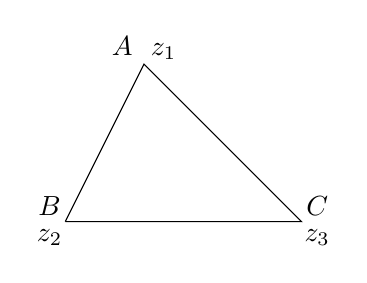
\begin{tikzpicture}
				\draw (0,0) node [xshift=-2mm,yshift=2mm] {$B$}node [xshift=-2mm,yshift=-2mm] {$z_2$}-- (3,0)node [xshift=2mm,yshift=2mm] {$C$} node [xshift=2mm,yshift=-2mm]{$z_3$} -- (1,2) node [yshift=2mm] {$A$ \ $z_1$}-- (0,0);
			\end{tikzpicture}
		\end{center}
	The angle between the sides $AB$ and $AC$ defined to be the angle between the sides in the anti clockwise direction. Hence we can define the angle $$\angle A= \Im \log \lt( \frac{z_3-z_1}{z_2-z_1} \rt)=\Im \lt(\log(z_3-z_1)-\log(z_2-z_1)  \rt) = \Im \log(z_3-z_1)-\Im\log(z_2-z_1)  $$Therefore for other angles we have $$\angle B=\Im\log \lt( \frac{z_1-z_2}{z_3-z_2} \rt)=\Im \log(z_1-z_2)-\Im\log(z_3-z_2)$$  $$\angle C=\Im\log \lt( \frac{z_2-z_3}{z_1-z_3} \rt)=\Im \log(z_2-z_3)-\Im\log(z_1-z_3)$$Therefore \begin{align*}
		\angle A+\angle B+\angle C & =  \Im \log \lt( \frac{z_3-z_1}{z_2-z_1} \rt) + \Im\log \lt( \frac{z_1-z_2}{z_3-z_2} \rt)+\Im\log \lt( \frac{z_2-z_3}{z_1-z_3} \rt) \\
		& = \Im \log \lt( \frac{z_3-z_1}{z_2-z_1} \, \frac{z_1-z_2}{z_3-z_2} \,   \frac{z_2-z_3}{z_1-z_3}  \rt)\\
		& = \Im \log \lt( \frac{z_1-z_2}{z_2-z_1} \, \frac{z_2-z_3}{z_3-z_2} \,   \frac{z_3-z_1}{z_1-z_3}  \rt)\\
		&= \Im \log \lt((-1)^3\rt)=\Im \log (-1)=\pi
	\end{align*}
		
	}
		%%%%%%%%%%%%%%%%%%%%%%%%%%%%%%%%%%%%%%%%%%%%%%%%%%%%%%%%%%%%%%%%%%%%%%%%%
	% Problem 7
	%%%%%%%%%%%%%%%%%%%%%%%%%%%%%%%%%%%%%%%%%%%%%%%%%%%%%%%%%%%%%%%%%%%%%%%%%
	
	\begin{problem}{%problem statement
			Ahlfors Page 72: Problem 1
		}{p5% problem reference text
		}
		%Problem
		Give a precise definition of a single-valued branch of $\sqrt{a+z}+\sqrt{1-z}$ in a suitable region, and prove that it is analytic.
	\end{problem}
	
	\solve{
		%Solution
	We recall that for $\sqrt{z}$ we choose the region $\Omega$ which is the complement of the negative real axis $x \leq 0$, $y = 0$. Hence, to define $\sqrt{1 + z}$ we should choose $\Omega_1$ as the complement of $x \leq -1$, $y = 0$ and for $\sqrt{1 - z}$ we should choose $\Omega_2$ as the complement of $1 \leq x$, $y = 0$. In total, to define $\sqrt{1 + z} + \sqrt{1 - z}$ we choose the region $\Omega = \Omega_1 \cap \Omega_2$. This is actually the same region used in	defining $\arccos z$. The branch chosen is that which has positive real part. As simple transformations of $\sqrt{z}$ in an analytic region, it follows that $\sqrt{1 + z} + \sqrt{1 - z}$ is analytic.
	}
\pagebreak
	
		%%%%%%%%%%%%%%%%%%%%%%%%%%%%%%%%%%%%%%%%%%%%%%%%%%%%%%%%%%%%%%%%%%%%%%%%%
	% Problem 8
	%%%%%%%%%%%%%%%%%%%%%%%%%%%%%%%%%%%%%%%%%%%%%%%%%%%%%%%%%%%%%%%%%%%%%%%%%
	
	\begin{problem}{%problem statement
			Ahlfors Page 72: Problem 3
		}{p5% problem reference text
		}
		%Problem		
	Suppose that $f(z)$ is analytic and satisfies the condition $|f^2(z)-1|<1$  in a region $\Omega$.  Show that either $\Re f(z) > 0$  or $\Re f(z) < 0$  through out  $\Omega$
	\end{problem}
	
	\solve{
		%Solution
		Suppose $\Re f(z) = 0$ at a point $z \in \Omega$. Then $f(z) = iy^2$ for some $y \in \bbR$, and thus
		$f(z)^2 = -y^2$. By the condition $|f(z)^2 -1| < 1$ we have $| -y^2 -1| < 1$ and thus $|y^2 + 1| < 1$.
		This is clearly impossible, so that $\Re f(z) \neq  0$ throughout $\Omega$. But, $\Re f(z)$ is continuous and $\Omega$ is connected, so either $\Re f(z) > 0$ or $\Re f(z) <0$.
	
	}
		%%%%%%%%%%%%%%%%%%%%%%%%%%%%%%%%%%%%%%%%%%%%%%%%%%%%%%%%%%%%%%%%%%%%%%%%%
	% Problem 9
	%%%%%%%%%%%%%%%%%%%%%%%%%%%%%%%%%%%%%%%%%%%%%%%%%%%%%%%%%%%%%%%%%%%%%%%%%
	\begin{problem}{%problem statement
			Ahlfors Page 78: Problem 1
		}{p5% problem reference text
		}
		%Problem		
		Prove that the reflection $z \to \overline{z}$ is not a linear transformation

	\end{problem}
	
	\solve{
		%Solution
		Suppose $\varphi(z):z\mapsto \overline{z}$ is a linear fractional transformation, and thus it must be of the form	$$	\overline{z}=\varphi(z)=\frac{a z+b}{c z+d}, \quad \forall\ z \in \mathbb{C}$$	Note that if $\Im z=0$ then $\overline{z}=z$. In particular,
		$$	0 \mapsto 0\implies \varphi(0)=\frac{b}{d}=0 \implies b=0 	$$
		Plugging in different values yields
		\begin{align*}
			1&  \mapsto \varphi(1)=\frac{a}{c+d} =1 \\
			-1&  \mapsto \varphi(-1)=\frac{-a}{-c+d} =-1
		\end{align*}
			Or,
		\begin{align*}
			c+d  =a \\
			d-c  =a
		\end{align*}
		Thus, $a=d$ and hence $c=0$. But then we have $$\overline{z}=\frac{a z}{d}=z$$Hence contradiction. $\varphi$ is not linear transformation
	 	}
		
	%%%%%%%%%%%%%%%%%%%%%%%%%%%%%%%%%%%%%%%%%%%%%%%%%%%%%%%%%%%%%%%%%%%%%%%%%
	% Problem 10
	%%%%%%%%%%%%%%%%%%%%%%%%%%%%%%%%%%%%%%%%%%%%%%%%%%%%%%%%%%%%%%%%%%%%%%%%%
	
	\begin{problem}{%problem statement
			Ahlfors Page 78: Problem 2
		}{p5% problem reference text
		}
		%Problem		
		If $$T_{1}z=\frac{z+2}{z+3}\qquad T_{2}z=\frac{z}{z+1}$$Find $T_1T_{2}z$, $T_{2}T_{1}z$, $T_1^{-1}T_{2}z$
		
	\end{problem}
	
	\solve{
		%Solution
		Here we compute several compositions:
		\begin{align*}
			& T_1 T_2 z=\frac{\frac{z}{z+1}+2}{\frac{z}{z+1}+3}=\frac{\frac{3 z+2}{z+1}}{\frac{4 z+3}{z+1}}=\frac{3 z+2}{4 z+3} \\
			& T_2 T_2 z=\frac{\frac{z+2}{z+3}}{\frac{z+2}{z+3}+1}=\frac{\frac{z+2}{z+3}}{\frac{2 z+5}{z+3}}=\frac{z+2}{2 z+5}
		\end{align*}
	Now note that$$	T_1^{-1}(w)=\frac{3 w-2}{1-w}$$	Thus,
		$$
		T_1^{-1} T_2 z=\frac{3 \frac{z}{z+1}-2}{1-\frac{z}{z+1}}=\frac{z-2}{1}=z-2
		$$
		
	}
	%%%%%%%%%%%%%%%%%%%%%%%%%%%%%%%%%%%%%%%%%%%%%%%%%%%%%%%%%%%%%%%%%%%%%%%%%
	% Problem 12
	%%%%%%%%%%%%%%%%%%%%%%%%%%%%%%%%%%%%%%%%%%%%%%%%%%%%%%%%%%%%%%%%%%%%%%%%%
	
	\begin{problem}{%problem statement
			Ahlfors Page 78: Problem 3
		}{p5% problem reference text
		}
		%Problem		
		Prove that the most general transformation which leaves the origin fixed and preserves all distances is either a rotation or a rotation followed by reflexion in the real axis.
		
	\end{problem}
	
	\solve{
		%Solution
		Let $\varphi$ be a fractional linear transformation as given. Then, we have that $\varphi(0)=0$ and for any pair $(z, w) \in \mathbb{C} \times \mathbb{C}$ :
		$$
		|z-w|=|\varphi(z)-\varphi(w)|
		$$
		since we assume that $\varphi$ preserved distance under transformation. Since $\varphi$ is fractional linear transformation we have $$\varphi(z)=\frac{a z+b}{c z+d}$$ where $a, b, c, d\in \bbC$. The assumption that $0 \mapsto 0$ yields immediately
		$$
		0=\varphi(0)=\frac{b}{d}
		$$
		and thus we have $b=0$. Now, as $\varphi(0)=0$ we see
		$$
		|z|=|\varphi(z)-\varphi(0)|=|\varphi(z)-0|=\left|\frac{a z}{c z+d}\right|=|a| \cdot \frac{|z|}{|c z+d|}, \quad \forall z \in \mathbb{C}
		$$
		If $|a|=0$ i.e. $a=0$ then $\varphi(z)=0$. Otherwise $|a|>0$. then for all $z \in \mathbb{C}$ we must have
		$$
		\frac{|a|}{|c z+d|} =1 \text { in } \mathbb{C}
		$$
		This can only happen if the denominator is also constant and hence we conclude that we require additionally that $c=0$. We are left with $\frac{|a|}{|d|}=1$, or $|a|=|d|$. Hence $$\varphi(z)=\frac{az}{d}$$ where $\lt|\frac{a}{d}\rt|=1$. Let $k=\frac{a}{d}$. Then $$\varphi(z)=kz\qquad \text{where }|k|=1$$Clearly $\varphi$ is a rotation.
		
	}
		
	%%%%%%%%%%%%%%%%%%%%%%%%%%%%%%%%%%%%%%%%%%%%%%%%%%%%%%%%%%%%%%%%%%%%%%%%%
	% Problem 13
	%%%%%%%%%%%%%%%%%%%%%%%%%%%%%%%%%%%%%%%%%%%%%%%%%%%%%%%%%%%%%%%%%%%%%%%%%
	
	\begin{problem}{%problem statement
			Ahlfors Page 78: Problem 4
		}{p5% problem reference text
		}
		%Problem		
		 Show that any linear transformation which transforms the real axis into itself can be written with real coefficients.
		
	\end{problem}
	
	\solve{
		%Solution
		Let $\varphi(z)$ be a linear transformation with the additional restriction that $\varphi(z) \in \mathbb{R}$ whenever $z \in \mathbb{R}$. Hence
		$$
		\varphi(z)=\frac{a z+b}{c z+d}
		$$
		for $a, b, c, d \in \mathbb{C}$. We will now find $\alpha, \beta, \gamma, \delta \in \mathbb{R}$ so that $\varphi(z)=\frac{\alpha z+\beta}{\gamma z+\delta}$. We need to distinguish separate cases:
		\subsection*{If $\boldsymbol{a \neq 0}$ :}
		$$
		\varphi(z)=\frac{a z+b}{c z+d} \cdot \frac{\overline{a}}{\overline{a}}=\frac{a^{\prime} z+b^{\prime}}{c^{\prime} z+d^{\prime}}, \quad a^{\prime} \in \mathbb{R}
		$$
		The important thing to observe is that we will then have $\Im a'=0$, i.e $a \in \mathbb{R}$. We now have a representation
		$$
		\varphi(z)=\frac{a' z+b'}{c' z+d'}, \quad a' \in \mathbb{R}
		$$
		In the above we see that $z\to\infty \implies \phi(\infty)= \frac{a'}{c'}$ implying that $c' \in \mathbb{R}$ as well as $a'$. The transformation has an inverse
		$$
		\varphi^{-1}(z)=\frac{d' z-b'}{a'-c' z}
		$$
		If $d'=0$ then taking $z=0$ we see $\varphi(0)=b$ and hence achieve $b' \in \mathbb{R}$. We now need to show that the same holds whenever $d '\neq 0$. In the above we see that $z\to\infty \implies \varphi^{-1}(\infty)= -\frac{d'}{c'}$ implying that $d' \in \mathbb{R}$ as well as $c'$.
		$$
		\varphi(0)= \frac{b'}{d'} \in \mathbb{R} \Longrightarrow b' \in \mathbb{R} 
		$$
		\subsection*{If $\boldsymbol{a = 0}$ :}\parinf
		If $a=0$ then we have $\varphi(z)=\frac{b}{c z+d}$. Here if $b=0$ we have  $\varphi(z)$ is non-invertible which is impossible. So  $$\varphi(z)=\frac{b}{c z+b} \cdot \frac{\overline{b}}{\overline{b}}$$ thus obtaining
		$$
		\varphi(z)=\frac{b'}{c' z+d'}, \quad b' \in \mathbb{R}
		$$
		Taking $z=0$ we see that $\varphi(0)= \frac{b'}{d'}$. We then have $d' \in \mathbb{R}$. If we take $z=1$ then $$\varphi(1)=\frac{b'}{c'+d'}$$Since $b',d,\in\bbR$ if $c'\notin \bbR$ then $c'+d'\notin \bbR$ but $c'+d'\in\bbC$ hence $\frac{b'}{c'+d'}\notin \bbR$ but $\frac{b'}{c'+d'}'\in\bbC$. But $\varphi(1)\in\bbR$. So $c'\in \bbR$. 
		
		\parinn
		
		Hence $\varphi$ can be written with real coefficients
		
}
	

	
\end{document}
